%%%%%%%%%%%%%%%%%%%%%%% file template.tex %%%%%%%%%%%%%%%%%%%%%%%%%
%
% This is a general template file for the LaTeX package SVJour3
% for Springer journals.          Springer Heidelberg 2010/09/16
%
% Copy it to a new file with a new name and use it as the basis
% for your article. Delete % signs as needed.
%
% This template includes a few options for different layouts and
% content for various journals. Please consult a previous issue of
% your journal as needed.
%
%%%%%%%%%%%%%%%%%%%%%%%%%%%%%%%%%%%%%%%%%%%%%%%%%%%%%%%%%%%%%%%%%%%
%
% First comes an example EPS file -- just ignore it and
% proceed on the \documentclass line
% your LaTeX will extract the file if required
\begin{filecontents*}{example.eps}
%!PS-Adobe-3.0 EPSF-3.0
%%BoundingBox: 19 19 221 221
%%CreationDate: Mon Sep 29 1997
%%Creator: programmed by hand (JK)
%%EndComments
gsave
newpath
  20 20 moveto
  20 220 lineto
  220 220 lineto
  220 20 lineto
closepath
2 setlinewidth
gsave
  .4 setgray fill
grestore
stroke
grestore
\end{filecontents*}
%
\RequirePackage{fix-cm}
%
%\documentclass{svjour3}                     % onecolumn (standard format)
%\documentclass[smallcondensed]{svjour3}     % onecolumn (ditto)
\documentclass[smallextended]{svjour3}       % onecolumn (second format)
%\documentclass[twocolumn]{svjour3}          % twocolumn
%
\smartqed  % flush right qed marks, e.g. at end of proof
%
\usepackage{graphicx,epsfig,subfigure,caption}
%
% \usepackage{mathptmx}      % use Times fonts if available on your TeX system
%
% insert here the call for the packages your document requires
%\usepackage{latexsym}
% etc.
%
% please place your own definitions here and don't use \def but
% \newcommand{}{}
%
% Insert the name of "your journal" with
% \journalname{myjournal}
%
\begin{document}

\title{Spatial features in POI classification%\thanks{Grants or other notes
%about the article that should go on the front page should be
%placed here. General acknowledgments should be placed at the end of the article.}
}
%\subtitle{Do you have a subtitle?\\ If so, write it here}

%\titlerunning{Short form of title}        % if too long for running head

\author{First Author         \and
        Second Author %etc.
}

%\authorrunning{Short form of author list} % if too long for running head

\institute{F. Author \at
              first address \\
              Tel.: +123-45-678910\\
              Fax: +123-45-678910\\
              \email{fauthor@example.com}           %  \\
%             \emph{Present address:} of F. Author  %  if needed
           \and
           S. Author \at
              second address
}

\date{Received: date / Accepted: date}
% The correct dates will be entered by the editor


\maketitle

\begin{abstract}
Insert your abstract here. Include keywords, PACS and mathematical
subject classification numbers as needed.
\keywords{First keyword \and Second keyword \and More}
% \PACS{PACS code1 \and PACS code2 \and more}
% \subclass{MSC code1 \and MSC code2 \and more}
\end{abstract}

%\IEEEraisesectionheading{
% %\IEEEraisesectionheading{
% %\IEEEraisesectionheading{
% \input{intro}
\section{Introduction}\label{sec:intro}
 %}
% \section{Introduction}\label{sec:intro}

% \begin{enumerate}
% \item Motivation: application scenarios (with 1-2 running examples);
% \item Characteristics of the data sources and their challenges;
% \item Briefly introduce previous approaches to extract information 
% from images including setting the document zone, and their limitations.
% \item General flow of our approach (may give a diagram here)
% \end{enumerate}
% scenary

Due to ever evolving hardware and software, many medical images
such as electro-cardio graphs (ECGs), X-ray or ultrasound images  
are directly printed and stored in hard copy formats. 
% \KZ{Insert 4 example images here.}
%Examples are shown in \figref{fig:medicalImages}. 
% These images often contain a mix of graphics and text, which
% include parameter settings of the hardware, test measurements or simple
% diagnosis. 
These images often contain a mix of graphics and text, which 
include technical settings of the hardware used, test measurements or simple diagnoses.
Recently, there has been a growing demand for digitizing such 
medical information from paper media sources, especially legacy ones, or patients who want to keep track of these documents by themselves digitally. 
Apart from scanning the graphics into a digital format, extracting 
the semi-structured textual information is also an important part of
building electronic medical records for patients. 

%\begin{figure}[!htb]
%\centering
%\subfloat[ECG]{
%\label{fig:medicalimage:ecg}
%\epsfig{file=figure/17_ori.eps, width=0.4\columnwidth}
%}
%% \hfill
%\subfloat[MRI]{
%	\label{fig:medicalimage:mrt}
%	\epsfig{file=figure/MRI.eps, width=0.4\columnwidth}
%}
%\\
%\subfloat[X-RAY]{
%\label{fig:medicalimage:xray}
%\epsfig{file=figure/X-RAY.eps, width=0.4\columnwidth}
%}
%%\hfill
%\subfloat[EEG]{
%\label{fig:medicalimage:eeg}
%\epsfig{file=figure/EEG.eps, width=0.4\columnwidth}
%}
%\caption{Examples of Medical Images}
%\label{fig:medicalImages}
%\end{figure}

Optical character recognition (OCR)  \cite{mori1992historical,smith2007overview} is 
a traditional technique used to turn images of printed text into machine encoded
text. It is well researched and performs well on plain text 
documents such as novels and reports, for a variety of languages. 
%For example, Tesseract, which is one of 
%the most popular open source multilingual recognizers, logs an error 
%rate of 3.72\% for English words and 3.77\% for simplified 
%Chinese characters\cite{smith2009adapting}. 
%Google Books \cite{googlebooks} and Gutenberg \cite{gutenberg} are
%projects which have scanned a large number of paper books into text for free and open
%access. These projects made exclusive use of OCR for this conversion and 
%achieved high accuracy \cite{vincent2007google} \cite{lebert2008project}. 
% 99\% for Gutenberg project \cite{lebert2008project}. 
% \KZ{Give the accuracy of google and gutenberg if available.}


\begin{figure}[th]
\centering
\epsfig{file=figure/17_b.eps, width=0.8\columnwidth}
\caption{An ECG image with text area (red circle) of interest.}
\label{fig:ecgexample2}
\end{figure}

For a semi-structured medical image, such as 
\figref{fig:ecgexample2}, we would like to extract the attribute-value 
pairs (e.g., {\em Vent. rate = 63 bpm}) and possibly other values such as
date ({\em 18-Nov-2010}) and time ({\em 9:13:02}) since those values endow us with lots of information about the patient. 
Existing OCR software cannot extract such structured information in a straightforward 
fashion, 
but instead it produces rather convoluted results from the whole image, 
similar to those in \figref{fig:ocrre}, which was produced by Tesseract, 
a popular multi-lingual recognizers. 
% \KZ{Maybe include the x-y coordinate info in the output as well?}  

\begin{figure}[th]
\centering
\scriptsize
\begin{verbatim}
<p class="ocr_par" title="box 263 33 444 119">
   <span class="ocr_l" title="box 264 33 336 45">
       <span class="ocrx_w" title="box 264 33 299 45">Vcnt.</span> 
       <span class="ocrx_w" title="box 308 34 336 45">rule</span> 
   </span>
   <span class='ocr_l'>
       <span class="ocrx_w" title="box 264 51 283 64">PR</span> 
       <span class="ocrx_w" title="box 291 51 346 64">Interval</span> 
       <span class="ocrx_w" title="box 389 52 411 64">140</span> 
       <span class="ocrx_w" title="box 420 55 439 64">ms</span> 
   </span>
   ...
   </span>
</p>
<p class="ocr_p" dir="ltr">
   <span class="ocr_l">
       <span class="ocrx_w" title="box 396 33 411 45">53</span> 
       <span class="ocrx_w" title="box 420 33 449 48">bpm</span> 
   </span>
</p>
\end{verbatim}
\caption{Snippet OCR results in XML, input to our framework.}
\label{fig:ocrre}
\end{figure}


%\input{xmlre1}

%However, OCR alone does not work well on semi-structured text and hence
%can't be directly used for information extraction from the aforementioned
%medical images. \KZ{Give the reason here, perhaps because OCR models are
%largely Markov based? So semi-structured data breaks the flow of text.}
%When a medical image is input to an ordinary OCR software, the spatial 
%information of the text components is often lost or mixed with noises
%and errors.
%%The reason is OCR converts the whole images into text data, in which 
%%useful information often mix with noises and errors. 
%In this paper, we would like to extract the attribute-value pairs
%and possibly other values from \figref{fig:ecgexample1} 
%and \figref{fig:ecgexample2}. 
%% or medical ultrasonography report. 
%Such images contain lots of non-textual information or noises.

% example & ref
%\begin{figure}[ht]
%\centering
%\epsfig{file=figure/46.eps, width=0.8\columnwidth}
%\caption{ECG Images From Printer1}
%\label{fig:ecgexample1}
%\end{figure}

% \begin{figure}[ht]
% \centering
% \subfloat[Printer1]{
% \label{fig:ecgexample:a}
% \epsfig{file=figure/46.eps, width=0.48\columnwidth}
% }
% \hfill
% \subfloat[Printer2]{
% \label{fig:ecgexample:b}
% \epsfig{file=figure/17.eps, width=0.48\columnwidth}
% }
% \caption{ECG images from two different printers}
% \label{fig:ecgexample}
% \end{figure}

Also, errors in the OCR text \cite{darwish2007error,taghva1996evaluation} will greatly affect the effectiveness 
of other related tasks. Much work has been done to improve the performance of the OCR\cite{kolak2003generative,cesarini1998informys}. However, there are still a number of significant challenges involved in extracting the information from medical images or OCR results in XML form. 

% First, medical images differ from pure text document in that them have 
% layout information. 
First, medical images differ from pure text documents in that 
they contain layout information.
Although most current OCR engines attempt to reproduce the physical 
layout of the text units, 
%(along with X-Y coordinates) and store them 
%in a special format such as XML 
% (\KZ{Better in the previous example})
such spatial
information is approximate and sometimes inaccurate, which is why neighboring
text blocks in \figref{fig:ecgexample2}, such as ``Vent. Rate'' and
``63 bpm'' were not automatically combined into the same XML block, but were 
rather far apart (shown in two different ``classes'') in \figref{fig:ocrre} made by OCR softwares. 
%Even for images produced by the same ECG printer, 
%the XML results can still be very different as 
The spatial layout is sensitive to many factors, such as accidental spots 
on the prints, color and contrast, or the angle of the camera. 
%In this case, solutions for other application domains, for example, the web, 
%are not well suited for information extraction from printed documents \cite{bartoli2014semisupervised}. With such inaccurate
%layout information produced by OCR,
%it is not easy to write a simple wrapper program to extract useful
%data from images, even if the images come from the same printer. 

%Writing a wrapper for each
%individual image would be tedious and counter-productive. Therefore,
%a mechanism that makes use of the spatial locality of the 
%text units in the image and 
%accommodates slight variations in the spatial layout would make the extraction
%more accurate and fault-tolerant.

%For example, \figref{fig:ocrre} is the simplified OCR results for the ECGs in 
%\figref{fig:ecgexample1} and \figref{fig:ecgexample2}. The results are in the XML format and have attritube named {\em class} 
%for layout information. Although these two images share similar format. 
%OCR engine generates different results in that it splits elements that 
%should be in the same line into two lines in the second example. 
%XML is sensitive to the layout results so it's hard to tolerate 
%all the layout results. 
%
% example check the term
% layout of ocr results can be restore, so why OCR engine don't restore the results 
% using the similar methods as we do?
% or the way we handle the layout problem is quite simple

% Delete for TIP
% Second, exiting OCR engines make heavy use of Markov properties such as n-grams
% since they primarily target the transformation of large body of text 
% \cite{kolak2003generative}. 
% % \KZ{Needs some refs here.}
% Unfortunately, the semi-structured texts in medical images are often 
% short and not even written in complete sentences, thus breaking Markov assumption. To make
% matters worse, medical images contain scientific language, which may be
% very different from the training corpora of these OCR engines.
% This explains why we see errors like ``Vcnt'' and ``rule'' 
% in \figref{fig:ocrre}. 
% %can't guarantee a perfect performance, which means 
% %there are errors and noises in the OCR results.
% %Many of them due to the fact that the data are no longer long, continous
% %sentences, thus breaking the Markov assumption made by many OCR algorithms. 
% %In \figref{fig:ocrresub:b}, ``Vent." is misrecognized as ``Vcnt.". 
% Without sufficient contextual information, OCR may also misrecognize a 
% digit as an alphabetic character, or as another similar digit. 
% Furthermore, the mix of text with images and formatting
% lines often confuses the OCR engine, which is more biased toward full
% text images.
% Exact pattern matching, as used in
% traditional information extraction, doesn't work with such noisy OCR output
% as it doesn't tolerate noises or errors in text. 
% %It's hard to autocorrect these errors 
% %because image quality is the most important affecting factor. 
% %The text we are processing can be full of no meaning words or 
% %strange numbers. 
% A fuzzy matching strategy is more desirable in this case. 
% % example, what are the traditional IEs

Second, there are many types of medical images, resulting from a variety of
medical tests. Different equipments for the same test can produce vastly 
different images. Writing individual extraction wrappers 
for the OCR outputs of all these formats is tedious and inefficient, 
and difficult for non-programmers.
%not to mention that there are significant programming barriers for 
%writing these wrappers, especially for the medical professionals who are the
%end users of these extraction results. 
%A more user-friendly approach enabling users to specify such extraction requirements would be preferred. 
%There are various kinds of medical images, such as electrocardiograph report, 
%medical ultrasonography report, etc. 
%However the basic measures for each type of medical test (e.g., ECG), 
%are very similar from machine to machine. Only the layouts are 
%different. 
% example medical images

Finally, most off-the-shelf OCR programs are pre-trained with specific 
recognition models, which may not be suitable for the extraction of 
%medical images.
%Furthermore, changes in imaging equipment technology over time may produce 
%different formats, layout, or terminology, rendering existing OCR models 
%obsolete. 
Re-training the models requires a large amount of labeled data, which may
not be available. 
%Incremental training as more labeled data arrives
%is currently not supported by any OCR product.    

%There have been some limited attempts to address some of the above challenges. 
%One solution is a plugin of an OCR program that allows the user to specify 
%target zones of interest in the image to be extracted. The zones specified for
%one image can be applied to images with slight variations by adjusting against
%a fixed reference point that is supposed to exist in all these images.
%% \KZ{I think the problem is not so much with the zones, because we also
%% have zones, but rather with the reference point.}
%% \JY{}
%% example products
%% http://www.square-9.com/automated-data-extraction-optical-character-recognition
%The problem with this solution is its high reliance on the OCR zones  
%established by the user. The performance of the results is affected by the 
%accuracy of the zones. If the zones are too big, the results will be full of 
%noise. If the zones are too small, results will miss something. 
%
%Another solution involves using the page layout analysis technique. The page layout 
%analysis technique is used to determine where the text 
%resides on a page \cite{o1993document}, 
%% \KZ{This page layout analysis approach is not clearly described. I don't understand after reading this paragraph.}
%% By using page layout analysis technique, the hierarchy of physical components 
%% can be generated and to match with the hierarchy of logical components, which 
%% is predefined. 
%this includes identifying and categorizing the 
%regions of interest in the scanned image of a text document. 
%Typically, the first step is to segment text zones from 
%non-textual zones and arrange them in their original order. 
%Then in order to analyze the logical roles of the text zones 
%(titles, captions, footnotes, etc.), logical layout analysis 
%is used for labeling the semantics of the text zones.
%Generally, page layout analysis is used for documents. The problem with applying 
%such a technique on medical images is that it creates so much noises 
%that performance is ultimately affected. 
%For medical imaging reports like ECG, useful information is often 
%found in the small components of the image, while most of the images are 
%read as noises. 
% check paper and more description, weakness, ref

%In this paper, 
%we propose a spatial data description language, which borrows its syntax from
%PADS \cite{fisher+:pads}, an ad hoc data processing language, 
%for describing semi-structured data in medical images. 
%% ref
%We call this language OCR description language, or ODL. 
%ODL is designed for extracting and parsing semi-structured text data 
%from images. We believe that  information extraction from those data in ODL form may be much easier than extracting information from rough data or data in XML form, which means that our preprocessing part proves to be necessary.
%%An example ODL description for the image in 
%%\figref{fig:ecgexample2} is shown in 
%%\figref{fig:description}. \KZ{Make this description two column, and give
%%some brief explanation of this description here.} 
%%The parsing result of this description is shown
%%in \figref{fig:parsing result}. \KZ{Give some explanation of the results,
%%otherwise don't show the result here. E.g., you need to explain what F, E, etc.
%%mean. You want to say that even though rate has been recognized as rule,
%%the bpm value was still extracted (but still wrong!).}
%% \KZ{I removed the preprocessing part, cos it's not important. Talk about it in
%% discussion sec.}
%%The our approach starts by preprocessing the images for text results.
%To use this framework, the user first describes the components in the image
%that he or she is interested in extracting. This includes constant strings
%and variables of different data types.   
%ODL allows the user to specify the approximate spatial layout and constraints on
%the data, e.g., integers within 
%a certain range, real numbers with certain decimal points, etc. 
%%This information is then as the key component in our fuzzy matching strategy. 
%The system then automatically generates a parser for these medical images.
%This parser uses the output XML from OCR with spatial information as an input, 
%and outputs a data structure with values extracted for each variables
%in the description, unless there is an unrecoverable error during the parsing process.
%In addition, approximate layout information and constraints are used in parsing process 
%to tolerate noises and small format variations in the input images. 
%%Specifically, this method could be called fuzzy matching, meaning that more candidates could be saved after the parsing process.  It's obvious that we may have a higher probability to obtain the accurate result if more candidates are kept so that fuzzy match should be used properly in our system.
%%An autogenerated parser based on the ODL description can release us from 
%%repetitive work. In this way, we turn the task of writing complex parsers 
%%into describing information on images.
%
%
%When users process many images of the same format, the system 
%automatically discovers parsing errors given the current model and 
%prompts the user to manually correct some of the frequent and prominent
%errors, which effectively serves as an online labeling function. 
%These incrementally labeled data are then used to update the parsing model. 


%It should be emphasized that the incremental learning model is very important in our whole system. Incremental learning is a machine learning paradigm where the learning process takes place whenever we have new examples or data added to our baisc data set, leading to a most striking difference between incremental learning and traditional machine learning: it does not assume the availability of a sufficient training set before the learning process. What incremental learning in our system is really impressive: it does not require a relatively good and stable training set at first time. In fact, it could improve the parsing result with even relatively rough training sets at first by absorbing new data or corrective information as time passes in dynamic systems. Besides, the process would be very effective when there are some new images coming in since training process would not learn from scratch, which might waste time and computation resource.

%At last, we propose an incrementally human correction framwork which can 
%make the best use of human correction to handle the misrecognition problem. 
% Base on our experiments on about 500 real life ECG images, 
% our approach achieves p1 and p2 after p3 times human correction. 
% experimental results

% \begin{figure}[h]
% \begin{lstlisting}
% Oenum str_month_t{
% 	"Jan", "Feb", "Mar", "Apr",
% 	"May", "Jun", "Jul", "Aug",
% 	"Sept", "Oct", "Nov", "Dec"
% };

% Ounion month_t{
% 	Oint(1,12)	num;
% 	str_month_t	str;
% };

% Ostruct time_t{
% 	Oint(1,31)	day;
% 	"-";
% 	month_t	month;
% 	"-";
% 	Oint	year;
% };

% Ostruct triple_t{
% 	"Vent.";
% 	hskip(\s)	skip1;
% 	"rate";
% 	Oint x;
% 	"bpm";
% 	vskip(\n)	skip2;
% };

% Oscource Ostruct entry_t{
% 	time_t(<-,-,-,0.3l>) t;
% 	triple_t(<0.1w,-,0.5w,->) d;
% };
% \end{lstlisting}
% \caption{Description}\label{fig:description}
% \end{figure}


In order to solve above problems, We design a system which makes three main contributions:
\begin{enumerate}
\item Based on some previous work on data description language \cite{lamport1986document,taft1999post,fisher+:pads},we design a new declarative spatial data description language called \textit{OCR description language}, or ODL,
which allows users to specify spatial and data constraints in medical 
images(\secref{sec:syntax});
\item We propose a noise-tolerant parser which takes OCR results
the ODL description as input and outputs a data structure with values 
extracted for each variables in the description (\secref{sec:semantics});
\item We propose an incremental manual correction 
framework\cite{von2008recaptcha,zhu2012learnpads++}, which 
takes advantage of user corrections  and improves the productivity
significantly (\secref{sec:correction}).
%To be more specific, the framework improves the traditional machine learning methods by using a incremental learning process to avoid starting from scratch when we are trying to apply human corrections in the system. That means the framework would be more effective than most corrective systems.
\end{enumerate}


\section{Introduction}\label{sec:intro}
 %}
% \section{Introduction}\label{sec:intro}

% \begin{enumerate}
% \item Motivation: application scenarios (with 1-2 running examples);
% \item Characteristics of the data sources and their challenges;
% \item Briefly introduce previous approaches to extract information 
% from images including setting the document zone, and their limitations.
% \item General flow of our approach (may give a diagram here)
% \end{enumerate}
% scenary

Due to ever evolving hardware and software, many medical images
such as electro-cardio graphs (ECGs), X-ray or ultrasound images  
are directly printed and stored in hard copy formats. 
% \KZ{Insert 4 example images here.}
%Examples are shown in \figref{fig:medicalImages}. 
% These images often contain a mix of graphics and text, which
% include parameter settings of the hardware, test measurements or simple
% diagnosis. 
These images often contain a mix of graphics and text, which 
include technical settings of the hardware used, test measurements or simple diagnoses.
Recently, there has been a growing demand for digitizing such 
medical information from paper media sources, especially legacy ones, or patients who want to keep track of these documents by themselves digitally. 
Apart from scanning the graphics into a digital format, extracting 
the semi-structured textual information is also an important part of
building electronic medical records for patients. 

%\begin{figure}[!htb]
%\centering
%\subfloat[ECG]{
%\label{fig:medicalimage:ecg}
%\epsfig{file=figure/17_ori.eps, width=0.4\columnwidth}
%}
%% \hfill
%\subfloat[MRI]{
%	\label{fig:medicalimage:mrt}
%	\epsfig{file=figure/MRI.eps, width=0.4\columnwidth}
%}
%\\
%\subfloat[X-RAY]{
%\label{fig:medicalimage:xray}
%\epsfig{file=figure/X-RAY.eps, width=0.4\columnwidth}
%}
%%\hfill
%\subfloat[EEG]{
%\label{fig:medicalimage:eeg}
%\epsfig{file=figure/EEG.eps, width=0.4\columnwidth}
%}
%\caption{Examples of Medical Images}
%\label{fig:medicalImages}
%\end{figure}

Optical character recognition (OCR)  \cite{mori1992historical,smith2007overview} is 
a traditional technique used to turn images of printed text into machine encoded
text. It is well researched and performs well on plain text 
documents such as novels and reports, for a variety of languages. 
%For example, Tesseract, which is one of 
%the most popular open source multilingual recognizers, logs an error 
%rate of 3.72\% for English words and 3.77\% for simplified 
%Chinese characters\cite{smith2009adapting}. 
%Google Books \cite{googlebooks} and Gutenberg \cite{gutenberg} are
%projects which have scanned a large number of paper books into text for free and open
%access. These projects made exclusive use of OCR for this conversion and 
%achieved high accuracy \cite{vincent2007google} \cite{lebert2008project}. 
% 99\% for Gutenberg project \cite{lebert2008project}. 
% \KZ{Give the accuracy of google and gutenberg if available.}


\begin{figure}[th]
\centering
\epsfig{file=figure/17_b.eps, width=0.8\columnwidth}
\caption{An ECG image with text area (red circle) of interest.}
\label{fig:ecgexample2}
\end{figure}

For a semi-structured medical image, such as 
\figref{fig:ecgexample2}, we would like to extract the attribute-value 
pairs (e.g., {\em Vent. rate = 63 bpm}) and possibly other values such as
date ({\em 18-Nov-2010}) and time ({\em 9:13:02}) since those values endow us with lots of information about the patient. 
Existing OCR software cannot extract such structured information in a straightforward 
fashion, 
but instead it produces rather convoluted results from the whole image, 
similar to those in \figref{fig:ocrre}, which was produced by Tesseract, 
a popular multi-lingual recognizers. 
% \KZ{Maybe include the x-y coordinate info in the output as well?}  

\begin{figure}[th]
\centering
\scriptsize
\begin{verbatim}
<p class="ocr_par" title="box 263 33 444 119">
   <span class="ocr_l" title="box 264 33 336 45">
       <span class="ocrx_w" title="box 264 33 299 45">Vcnt.</span> 
       <span class="ocrx_w" title="box 308 34 336 45">rule</span> 
   </span>
   <span class='ocr_l'>
       <span class="ocrx_w" title="box 264 51 283 64">PR</span> 
       <span class="ocrx_w" title="box 291 51 346 64">Interval</span> 
       <span class="ocrx_w" title="box 389 52 411 64">140</span> 
       <span class="ocrx_w" title="box 420 55 439 64">ms</span> 
   </span>
   ...
   </span>
</p>
<p class="ocr_p" dir="ltr">
   <span class="ocr_l">
       <span class="ocrx_w" title="box 396 33 411 45">53</span> 
       <span class="ocrx_w" title="box 420 33 449 48">bpm</span> 
   </span>
</p>
\end{verbatim}
\caption{Snippet OCR results in XML, input to our framework.}
\label{fig:ocrre}
\end{figure}


%% \begin{figure}[ht]
% \centering
% \subfigure[]{
% \label{fig:subfig:a}
% \begin{minipage}[b]{0.2\textwidth}
%\newsavebox{\firstlisting}
%\begin{lrbox}{\firstlisting}% Store first listing
%\begin{lstlisting}
%<p class='ocr_par' dir='ltr'>
%   <span class='ocr_line' id='line_2'>
%       <span class='ocrx_word' id='word_6'>Vent.</span>
%       <span class='ocrx_word' id='word_7'>rate</span>
%       <span class='ocrx_word' id='word_8'>65</span>
%       <span class='ocrx_word' id='word_9'>bpm</span>
%   </span>
%   <span class='ocr_line' id='line_3'>
%       <span class='ocrx_word' id='word_14'>PR</span>
%       <span class='ocrx_word' id='word_15'>interval</span>
%       <span class='ocrx_word' id='word_16'>162</span>
%       <span class='ocrx_word' id='word_17'>ms</span>
%   </span>
%    ...
%</p>
%\end{lstlisting}
%\end{lrbox}
% \end{minipage}
% }
% \hspace[1in]
% \subfigure[]{
% % \label{fig:subfig:b}
% % \begin{minipage}[b]{0.2\textwidth}
\newsavebox{\secondlisting}
\begin{lrbox}{\secondlisting}
% \tiny
\begin{lstlisting}[basicstyle=\tiny,]
<p class="ocr_par" title="box 263 33 444 119">
   <span class="ocr_l" title="box 264 33 336 45">
       <span class="ocrx_w" title="box 264 33 299 45">Vcnt.</span>
       <span class="ocrx_w" title="box 308 34 336 45">rule</span>
   </span>
   <span class='ocr_l'>
       <span class="ocrx_w" title="box 264 51 283 64">PR</span>
       <span class="ocrx_w" title="box 291 51 346 64">Interval</span>
       <span class="ocrx_w" title="box 389 52 411 64">140</span>
       <span class="ocrx_w" title="box 420 55 439 64">ms</span>
   </span>
   ...
   </span>
</p>
<p class="ocr_p" dir="ltr">
   <span class="ocr_l">
       <span class="ocrx_w" title="box 396 33 411 45">53</span>
       <span class="ocrx_w" title="box 420 33 449 48">bpm</span>
   </span>
</p>
\end{lstlisting}
\end{lrbox}
% % \end{minipage}
% }

% \KZ{\figref{fig:ocrre} is output from what software? Tesseract?}
\begin{figure*}[th]
%\subfloat[Image From Printer1]{
%\label{fig:ocrresub:a}
%\scalebox{0.8}{\usebox{\firstlisting}}}
%\hfill
%\subfloat[Image From Printer2]{
\scalebox{1.6}{\usebox{\secondlisting}}
% \label{fig:ocrre}
\caption{A fragment of raw OCR results for ECG with layout information.}
%\caption{Simplified OCR Results in XML for an ECG with Layout Information}
%\label{fig:ocrresub:b}
\label{fig:running-xml}
\end{figure*}

% \lipsum[2]


%However, OCR alone does not work well on semi-structured text and hence
%can't be directly used for information extraction from the aforementioned
%medical images. \KZ{Give the reason here, perhaps because OCR models are
%largely Markov based? So semi-structured data breaks the flow of text.}
%When a medical image is input to an ordinary OCR software, the spatial 
%information of the text components is often lost or mixed with noises
%and errors.
%%The reason is OCR converts the whole images into text data, in which 
%%useful information often mix with noises and errors. 
%In this paper, we would like to extract the attribute-value pairs
%and possibly other values from \figref{fig:ecgexample1} 
%and \figref{fig:ecgexample2}. 
%% or medical ultrasonography report. 
%Such images contain lots of non-textual information or noises.

% example & ref
%\begin{figure}[ht]
%\centering
%\epsfig{file=figure/46.eps, width=0.8\columnwidth}
%\caption{ECG Images From Printer1}
%\label{fig:ecgexample1}
%\end{figure}

% \begin{figure}[ht]
% \centering
% \subfloat[Printer1]{
% \label{fig:ecgexample:a}
% \epsfig{file=figure/46.eps, width=0.48\columnwidth}
% }
% \hfill
% \subfloat[Printer2]{
% \label{fig:ecgexample:b}
% \epsfig{file=figure/17.eps, width=0.48\columnwidth}
% }
% \caption{ECG images from two different printers}
% \label{fig:ecgexample}
% \end{figure}

Also, errors in the OCR text \cite{darwish2007error,taghva1996evaluation} will greatly affect the effectiveness 
of other related tasks. Much work has been done to improve the performance of the OCR\cite{kolak2003generative,cesarini1998informys}. However, there are still a number of significant challenges involved in extracting the information from medical images or OCR results in XML form. 

% First, medical images differ from pure text document in that them have 
% layout information. 
First, medical images differ from pure text documents in that 
they contain layout information.
Although most current OCR engines attempt to reproduce the physical 
layout of the text units, 
%(along with X-Y coordinates) and store them 
%in a special format such as XML 
% (\KZ{Better in the previous example})
such spatial
information is approximate and sometimes inaccurate, which is why neighboring
text blocks in \figref{fig:ecgexample2}, such as ``Vent. Rate'' and
``63 bpm'' were not automatically combined into the same XML block, but were 
rather far apart (shown in two different ``classes'') in \figref{fig:ocrre} made by OCR softwares. 
%Even for images produced by the same ECG printer, 
%the XML results can still be very different as 
The spatial layout is sensitive to many factors, such as accidental spots 
on the prints, color and contrast, or the angle of the camera. 
%In this case, solutions for other application domains, for example, the web, 
%are not well suited for information extraction from printed documents \cite{bartoli2014semisupervised}. With such inaccurate
%layout information produced by OCR,
%it is not easy to write a simple wrapper program to extract useful
%data from images, even if the images come from the same printer. 

%Writing a wrapper for each
%individual image would be tedious and counter-productive. Therefore,
%a mechanism that makes use of the spatial locality of the 
%text units in the image and 
%accommodates slight variations in the spatial layout would make the extraction
%more accurate and fault-tolerant.

%For example, \figref{fig:ocrre} is the simplified OCR results for the ECGs in 
%\figref{fig:ecgexample1} and \figref{fig:ecgexample2}. The results are in the XML format and have attritube named {\em class} 
%for layout information. Although these two images share similar format. 
%OCR engine generates different results in that it splits elements that 
%should be in the same line into two lines in the second example. 
%XML is sensitive to the layout results so it's hard to tolerate 
%all the layout results. 
%
% example check the term
% layout of ocr results can be restore, so why OCR engine don't restore the results 
% using the similar methods as we do?
% or the way we handle the layout problem is quite simple

% Delete for TIP
% Second, exiting OCR engines make heavy use of Markov properties such as n-grams
% since they primarily target the transformation of large body of text 
% \cite{kolak2003generative}. 
% % \KZ{Needs some refs here.}
% Unfortunately, the semi-structured texts in medical images are often 
% short and not even written in complete sentences, thus breaking Markov assumption. To make
% matters worse, medical images contain scientific language, which may be
% very different from the training corpora of these OCR engines.
% This explains why we see errors like ``Vcnt'' and ``rule'' 
% in \figref{fig:ocrre}. 
% %can't guarantee a perfect performance, which means 
% %there are errors and noises in the OCR results.
% %Many of them due to the fact that the data are no longer long, continous
% %sentences, thus breaking the Markov assumption made by many OCR algorithms. 
% %In \figref{fig:ocrresub:b}, ``Vent." is misrecognized as ``Vcnt.". 
% Without sufficient contextual information, OCR may also misrecognize a 
% digit as an alphabetic character, or as another similar digit. 
% Furthermore, the mix of text with images and formatting
% lines often confuses the OCR engine, which is more biased toward full
% text images.
% Exact pattern matching, as used in
% traditional information extraction, doesn't work with such noisy OCR output
% as it doesn't tolerate noises or errors in text. 
% %It's hard to autocorrect these errors 
% %because image quality is the most important affecting factor. 
% %The text we are processing can be full of no meaning words or 
% %strange numbers. 
% A fuzzy matching strategy is more desirable in this case. 
% % example, what are the traditional IEs

Second, there are many types of medical images, resulting from a variety of
medical tests. Different equipments for the same test can produce vastly 
different images. Writing individual extraction wrappers 
for the OCR outputs of all these formats is tedious and inefficient, 
and difficult for non-programmers.
%not to mention that there are significant programming barriers for 
%writing these wrappers, especially for the medical professionals who are the
%end users of these extraction results. 
%A more user-friendly approach enabling users to specify such extraction requirements would be preferred. 
%There are various kinds of medical images, such as electrocardiograph report, 
%medical ultrasonography report, etc. 
%However the basic measures for each type of medical test (e.g., ECG), 
%are very similar from machine to machine. Only the layouts are 
%different. 
% example medical images

Finally, most off-the-shelf OCR programs are pre-trained with specific 
recognition models, which may not be suitable for the extraction of 
%medical images.
%Furthermore, changes in imaging equipment technology over time may produce 
%different formats, layout, or terminology, rendering existing OCR models 
%obsolete. 
Re-training the models requires a large amount of labeled data, which may
not be available. 
%Incremental training as more labeled data arrives
%is currently not supported by any OCR product.    

%There have been some limited attempts to address some of the above challenges. 
%One solution is a plugin of an OCR program that allows the user to specify 
%target zones of interest in the image to be extracted. The zones specified for
%one image can be applied to images with slight variations by adjusting against
%a fixed reference point that is supposed to exist in all these images.
%% \KZ{I think the problem is not so much with the zones, because we also
%% have zones, but rather with the reference point.}
%% \JY{}
%% example products
%% http://www.square-9.com/automated-data-extraction-optical-character-recognition
%The problem with this solution is its high reliance on the OCR zones  
%established by the user. The performance of the results is affected by the 
%accuracy of the zones. If the zones are too big, the results will be full of 
%noise. If the zones are too small, results will miss something. 
%
%Another solution involves using the page layout analysis technique. The page layout 
%analysis technique is used to determine where the text 
%resides on a page \cite{o1993document}, 
%% \KZ{This page layout analysis approach is not clearly described. I don't understand after reading this paragraph.}
%% By using page layout analysis technique, the hierarchy of physical components 
%% can be generated and to match with the hierarchy of logical components, which 
%% is predefined. 
%this includes identifying and categorizing the 
%regions of interest in the scanned image of a text document. 
%Typically, the first step is to segment text zones from 
%non-textual zones and arrange them in their original order. 
%Then in order to analyze the logical roles of the text zones 
%(titles, captions, footnotes, etc.), logical layout analysis 
%is used for labeling the semantics of the text zones.
%Generally, page layout analysis is used for documents. The problem with applying 
%such a technique on medical images is that it creates so much noises 
%that performance is ultimately affected. 
%For medical imaging reports like ECG, useful information is often 
%found in the small components of the image, while most of the images are 
%read as noises. 
% check paper and more description, weakness, ref

%In this paper, 
%we propose a spatial data description language, which borrows its syntax from
%PADS \cite{fisher+:pads}, an ad hoc data processing language, 
%for describing semi-structured data in medical images. 
%% ref
%We call this language OCR description language, or ODL. 
%ODL is designed for extracting and parsing semi-structured text data 
%from images. We believe that  information extraction from those data in ODL form may be much easier than extracting information from rough data or data in XML form, which means that our preprocessing part proves to be necessary.
%%An example ODL description for the image in 
%%\figref{fig:ecgexample2} is shown in 
%%\figref{fig:description}. \KZ{Make this description two column, and give
%%some brief explanation of this description here.} 
%%The parsing result of this description is shown
%%in \figref{fig:parsing result}. \KZ{Give some explanation of the results,
%%otherwise don't show the result here. E.g., you need to explain what F, E, etc.
%%mean. You want to say that even though rate has been recognized as rule,
%%the bpm value was still extracted (but still wrong!).}
%% \KZ{I removed the preprocessing part, cos it's not important. Talk about it in
%% discussion sec.}
%%The our approach starts by preprocessing the images for text results.
%To use this framework, the user first describes the components in the image
%that he or she is interested in extracting. This includes constant strings
%and variables of different data types.   
%ODL allows the user to specify the approximate spatial layout and constraints on
%the data, e.g., integers within 
%a certain range, real numbers with certain decimal points, etc. 
%%This information is then as the key component in our fuzzy matching strategy. 
%The system then automatically generates a parser for these medical images.
%This parser uses the output XML from OCR with spatial information as an input, 
%and outputs a data structure with values extracted for each variables
%in the description, unless there is an unrecoverable error during the parsing process.
%In addition, approximate layout information and constraints are used in parsing process 
%to tolerate noises and small format variations in the input images. 
%%Specifically, this method could be called fuzzy matching, meaning that more candidates could be saved after the parsing process.  It's obvious that we may have a higher probability to obtain the accurate result if more candidates are kept so that fuzzy match should be used properly in our system.
%%An autogenerated parser based on the ODL description can release us from 
%%repetitive work. In this way, we turn the task of writing complex parsers 
%%into describing information on images.
%
%
%When users process many images of the same format, the system 
%automatically discovers parsing errors given the current model and 
%prompts the user to manually correct some of the frequent and prominent
%errors, which effectively serves as an online labeling function. 
%These incrementally labeled data are then used to update the parsing model. 


%It should be emphasized that the incremental learning model is very important in our whole system. Incremental learning is a machine learning paradigm where the learning process takes place whenever we have new examples or data added to our baisc data set, leading to a most striking difference between incremental learning and traditional machine learning: it does not assume the availability of a sufficient training set before the learning process. What incremental learning in our system is really impressive: it does not require a relatively good and stable training set at first time. In fact, it could improve the parsing result with even relatively rough training sets at first by absorbing new data or corrective information as time passes in dynamic systems. Besides, the process would be very effective when there are some new images coming in since training process would not learn from scratch, which might waste time and computation resource.

%At last, we propose an incrementally human correction framwork which can 
%make the best use of human correction to handle the misrecognition problem. 
% Base on our experiments on about 500 real life ECG images, 
% our approach achieves p1 and p2 after p3 times human correction. 
% experimental results

% \begin{figure}[h]
% \begin{lstlisting}
% Oenum str_month_t{
% 	"Jan", "Feb", "Mar", "Apr",
% 	"May", "Jun", "Jul", "Aug",
% 	"Sept", "Oct", "Nov", "Dec"
% };

% Ounion month_t{
% 	Oint(1,12)	num;
% 	str_month_t	str;
% };

% Ostruct time_t{
% 	Oint(1,31)	day;
% 	"-";
% 	month_t	month;
% 	"-";
% 	Oint	year;
% };

% Ostruct triple_t{
% 	"Vent.";
% 	hskip(\s)	skip1;
% 	"rate";
% 	Oint x;
% 	"bpm";
% 	vskip(\n)	skip2;
% };

% Oscource Ostruct entry_t{
% 	time_t(<-,-,-,0.3l>) t;
% 	triple_t(<0.1w,-,0.5w,->) d;
% };
% \end{lstlisting}
% \caption{Description}\label{fig:description}
% \end{figure}


In order to solve above problems, We design a system which makes three main contributions:
\begin{enumerate}
\item Based on some previous work on data description language \cite{lamport1986document,taft1999post,fisher+:pads},we design a new declarative spatial data description language called \textit{OCR description language}, or ODL,
which allows users to specify spatial and data constraints in medical 
images(\secref{sec:syntax});
\item We propose a noise-tolerant parser which takes OCR results
the ODL description as input and outputs a data structure with values 
extracted for each variables in the description (\secref{sec:semantics});
\item We propose an incremental manual correction 
framework\cite{von2008recaptcha,zhu2012learnpads++}, which 
takes advantage of user corrections  and improves the productivity
significantly (\secref{sec:correction}).
%To be more specific, the framework improves the traditional machine learning methods by using a incremental learning process to avoid starting from scratch when we are trying to apply human corrections in the system. That means the framework would be more effective than most corrective systems.
\end{enumerate}


\section{Introduction}\label{sec:intro}
 %}
% \section{Introduction}\label{sec:intro}

% \begin{enumerate}
% \item Motivation: application scenarios (with 1-2 running examples);
% \item Characteristics of the data sources and their challenges;
% \item Briefly introduce previous approaches to extract information 
% from images including setting the document zone, and their limitations.
% \item General flow of our approach (may give a diagram here)
% \end{enumerate}
% scenary

Due to ever evolving hardware and software, many medical images
such as electro-cardio graphs (ECGs), X-ray or ultrasound images  
are directly printed and stored in hard copy formats. 
% \KZ{Insert 4 example images here.}
%Examples are shown in \figref{fig:medicalImages}. 
% These images often contain a mix of graphics and text, which
% include parameter settings of the hardware, test measurements or simple
% diagnosis. 
These images often contain a mix of graphics and text, which 
include technical settings of the hardware used, test measurements or simple diagnoses.
Recently, there has been a growing demand for digitizing such 
medical information from paper media sources, especially legacy ones, or patients who want to keep track of these documents by themselves digitally. 
Apart from scanning the graphics into a digital format, extracting 
the semi-structured textual information is also an important part of
building electronic medical records for patients. 

%\begin{figure}[!htb]
%\centering
%\subfloat[ECG]{
%\label{fig:medicalimage:ecg}
%\epsfig{file=figure/17_ori.eps, width=0.4\columnwidth}
%}
%% \hfill
%\subfloat[MRI]{
%	\label{fig:medicalimage:mrt}
%	\epsfig{file=figure/MRI.eps, width=0.4\columnwidth}
%}
%\\
%\subfloat[X-RAY]{
%\label{fig:medicalimage:xray}
%\epsfig{file=figure/X-RAY.eps, width=0.4\columnwidth}
%}
%%\hfill
%\subfloat[EEG]{
%\label{fig:medicalimage:eeg}
%\epsfig{file=figure/EEG.eps, width=0.4\columnwidth}
%}
%\caption{Examples of Medical Images}
%\label{fig:medicalImages}
%\end{figure}

Optical character recognition (OCR)  \cite{mori1992historical,smith2007overview} is 
a traditional technique used to turn images of printed text into machine encoded
text. It is well researched and performs well on plain text 
documents such as novels and reports, for a variety of languages. 
%For example, Tesseract, which is one of 
%the most popular open source multilingual recognizers, logs an error 
%rate of 3.72\% for English words and 3.77\% for simplified 
%Chinese characters\cite{smith2009adapting}. 
%Google Books \cite{googlebooks} and Gutenberg \cite{gutenberg} are
%projects which have scanned a large number of paper books into text for free and open
%access. These projects made exclusive use of OCR for this conversion and 
%achieved high accuracy \cite{vincent2007google} \cite{lebert2008project}. 
% 99\% for Gutenberg project \cite{lebert2008project}. 
% \KZ{Give the accuracy of google and gutenberg if available.}


\begin{figure}[th]
\centering
\epsfig{file=figure/17_b.eps, width=0.8\columnwidth}
\caption{An ECG image with text area (red circle) of interest.}
\label{fig:ecgexample2}
\end{figure}

For a semi-structured medical image, such as 
\figref{fig:ecgexample2}, we would like to extract the attribute-value 
pairs (e.g., {\em Vent. rate = 63 bpm}) and possibly other values such as
date ({\em 18-Nov-2010}) and time ({\em 9:13:02}) since those values endow us with lots of information about the patient. 
Existing OCR software cannot extract such structured information in a straightforward 
fashion, 
but instead it produces rather convoluted results from the whole image, 
similar to those in \figref{fig:ocrre}, which was produced by Tesseract, 
a popular multi-lingual recognizers. 
% \KZ{Maybe include the x-y coordinate info in the output as well?}  

\begin{figure}[th]
\centering
\scriptsize
\begin{verbatim}
<p class="ocr_par" title="box 263 33 444 119">
   <span class="ocr_l" title="box 264 33 336 45">
       <span class="ocrx_w" title="box 264 33 299 45">Vcnt.</span> 
       <span class="ocrx_w" title="box 308 34 336 45">rule</span> 
   </span>
   <span class='ocr_l'>
       <span class="ocrx_w" title="box 264 51 283 64">PR</span> 
       <span class="ocrx_w" title="box 291 51 346 64">Interval</span> 
       <span class="ocrx_w" title="box 389 52 411 64">140</span> 
       <span class="ocrx_w" title="box 420 55 439 64">ms</span> 
   </span>
   ...
   </span>
</p>
<p class="ocr_p" dir="ltr">
   <span class="ocr_l">
       <span class="ocrx_w" title="box 396 33 411 45">53</span> 
       <span class="ocrx_w" title="box 420 33 449 48">bpm</span> 
   </span>
</p>
\end{verbatim}
\caption{Snippet OCR results in XML, input to our framework.}
\label{fig:ocrre}
\end{figure}


%% \begin{figure}[ht]
% \centering
% \subfigure[]{
% \label{fig:subfig:a}
% \begin{minipage}[b]{0.2\textwidth}
%\newsavebox{\firstlisting}
%\begin{lrbox}{\firstlisting}% Store first listing
%\begin{lstlisting}
%<p class='ocr_par' dir='ltr'>
%   <span class='ocr_line' id='line_2'>
%       <span class='ocrx_word' id='word_6'>Vent.</span>
%       <span class='ocrx_word' id='word_7'>rate</span>
%       <span class='ocrx_word' id='word_8'>65</span>
%       <span class='ocrx_word' id='word_9'>bpm</span>
%   </span>
%   <span class='ocr_line' id='line_3'>
%       <span class='ocrx_word' id='word_14'>PR</span>
%       <span class='ocrx_word' id='word_15'>interval</span>
%       <span class='ocrx_word' id='word_16'>162</span>
%       <span class='ocrx_word' id='word_17'>ms</span>
%   </span>
%    ...
%</p>
%\end{lstlisting}
%\end{lrbox}
% \end{minipage}
% }
% \hspace[1in]
% \subfigure[]{
% % \label{fig:subfig:b}
% % \begin{minipage}[b]{0.2\textwidth}
\newsavebox{\secondlisting}
\begin{lrbox}{\secondlisting}
% \tiny
\begin{lstlisting}[basicstyle=\tiny,]
<p class="ocr_par" title="box 263 33 444 119">
   <span class="ocr_l" title="box 264 33 336 45">
       <span class="ocrx_w" title="box 264 33 299 45">Vcnt.</span>
       <span class="ocrx_w" title="box 308 34 336 45">rule</span>
   </span>
   <span class='ocr_l'>
       <span class="ocrx_w" title="box 264 51 283 64">PR</span>
       <span class="ocrx_w" title="box 291 51 346 64">Interval</span>
       <span class="ocrx_w" title="box 389 52 411 64">140</span>
       <span class="ocrx_w" title="box 420 55 439 64">ms</span>
   </span>
   ...
   </span>
</p>
<p class="ocr_p" dir="ltr">
   <span class="ocr_l">
       <span class="ocrx_w" title="box 396 33 411 45">53</span>
       <span class="ocrx_w" title="box 420 33 449 48">bpm</span>
   </span>
</p>
\end{lstlisting}
\end{lrbox}
% % \end{minipage}
% }

% \KZ{\figref{fig:ocrre} is output from what software? Tesseract?}
\begin{figure*}[th]
%\subfloat[Image From Printer1]{
%\label{fig:ocrresub:a}
%\scalebox{0.8}{\usebox{\firstlisting}}}
%\hfill
%\subfloat[Image From Printer2]{
\scalebox{1.6}{\usebox{\secondlisting}}
% \label{fig:ocrre}
\caption{A fragment of raw OCR results for ECG with layout information.}
%\caption{Simplified OCR Results in XML for an ECG with Layout Information}
%\label{fig:ocrresub:b}
\label{fig:running-xml}
\end{figure*}

% \lipsum[2]


%However, OCR alone does not work well on semi-structured text and hence
%can't be directly used for information extraction from the aforementioned
%medical images. \KZ{Give the reason here, perhaps because OCR models are
%largely Markov based? So semi-structured data breaks the flow of text.}
%When a medical image is input to an ordinary OCR software, the spatial 
%information of the text components is often lost or mixed with noises
%and errors.
%%The reason is OCR converts the whole images into text data, in which 
%%useful information often mix with noises and errors. 
%In this paper, we would like to extract the attribute-value pairs
%and possibly other values from \figref{fig:ecgexample1} 
%and \figref{fig:ecgexample2}. 
%% or medical ultrasonography report. 
%Such images contain lots of non-textual information or noises.

% example & ref
%\begin{figure}[ht]
%\centering
%\epsfig{file=figure/46.eps, width=0.8\columnwidth}
%\caption{ECG Images From Printer1}
%\label{fig:ecgexample1}
%\end{figure}

% \begin{figure}[ht]
% \centering
% \subfloat[Printer1]{
% \label{fig:ecgexample:a}
% \epsfig{file=figure/46.eps, width=0.48\columnwidth}
% }
% \hfill
% \subfloat[Printer2]{
% \label{fig:ecgexample:b}
% \epsfig{file=figure/17.eps, width=0.48\columnwidth}
% }
% \caption{ECG images from two different printers}
% \label{fig:ecgexample}
% \end{figure}

Also, errors in the OCR text \cite{darwish2007error,taghva1996evaluation} will greatly affect the effectiveness 
of other related tasks. Much work has been done to improve the performance of the OCR\cite{kolak2003generative,cesarini1998informys}. However, there are still a number of significant challenges involved in extracting the information from medical images or OCR results in XML form. 

% First, medical images differ from pure text document in that them have 
% layout information. 
First, medical images differ from pure text documents in that 
they contain layout information.
Although most current OCR engines attempt to reproduce the physical 
layout of the text units, 
%(along with X-Y coordinates) and store them 
%in a special format such as XML 
% (\KZ{Better in the previous example})
such spatial
information is approximate and sometimes inaccurate, which is why neighboring
text blocks in \figref{fig:ecgexample2}, such as ``Vent. Rate'' and
``63 bpm'' were not automatically combined into the same XML block, but were 
rather far apart (shown in two different ``classes'') in \figref{fig:ocrre} made by OCR softwares. 
%Even for images produced by the same ECG printer, 
%the XML results can still be very different as 
The spatial layout is sensitive to many factors, such as accidental spots 
on the prints, color and contrast, or the angle of the camera. 
%In this case, solutions for other application domains, for example, the web, 
%are not well suited for information extraction from printed documents \cite{bartoli2014semisupervised}. With such inaccurate
%layout information produced by OCR,
%it is not easy to write a simple wrapper program to extract useful
%data from images, even if the images come from the same printer. 

%Writing a wrapper for each
%individual image would be tedious and counter-productive. Therefore,
%a mechanism that makes use of the spatial locality of the 
%text units in the image and 
%accommodates slight variations in the spatial layout would make the extraction
%more accurate and fault-tolerant.

%For example, \figref{fig:ocrre} is the simplified OCR results for the ECGs in 
%\figref{fig:ecgexample1} and \figref{fig:ecgexample2}. The results are in the XML format and have attritube named {\em class} 
%for layout information. Although these two images share similar format. 
%OCR engine generates different results in that it splits elements that 
%should be in the same line into two lines in the second example. 
%XML is sensitive to the layout results so it's hard to tolerate 
%all the layout results. 
%
% example check the term
% layout of ocr results can be restore, so why OCR engine don't restore the results 
% using the similar methods as we do?
% or the way we handle the layout problem is quite simple

% Delete for TIP
% Second, exiting OCR engines make heavy use of Markov properties such as n-grams
% since they primarily target the transformation of large body of text 
% \cite{kolak2003generative}. 
% % \KZ{Needs some refs here.}
% Unfortunately, the semi-structured texts in medical images are often 
% short and not even written in complete sentences, thus breaking Markov assumption. To make
% matters worse, medical images contain scientific language, which may be
% very different from the training corpora of these OCR engines.
% This explains why we see errors like ``Vcnt'' and ``rule'' 
% in \figref{fig:ocrre}. 
% %can't guarantee a perfect performance, which means 
% %there are errors and noises in the OCR results.
% %Many of them due to the fact that the data are no longer long, continous
% %sentences, thus breaking the Markov assumption made by many OCR algorithms. 
% %In \figref{fig:ocrresub:b}, ``Vent." is misrecognized as ``Vcnt.". 
% Without sufficient contextual information, OCR may also misrecognize a 
% digit as an alphabetic character, or as another similar digit. 
% Furthermore, the mix of text with images and formatting
% lines often confuses the OCR engine, which is more biased toward full
% text images.
% Exact pattern matching, as used in
% traditional information extraction, doesn't work with such noisy OCR output
% as it doesn't tolerate noises or errors in text. 
% %It's hard to autocorrect these errors 
% %because image quality is the most important affecting factor. 
% %The text we are processing can be full of no meaning words or 
% %strange numbers. 
% A fuzzy matching strategy is more desirable in this case. 
% % example, what are the traditional IEs

Second, there are many types of medical images, resulting from a variety of
medical tests. Different equipments for the same test can produce vastly 
different images. Writing individual extraction wrappers 
for the OCR outputs of all these formats is tedious and inefficient, 
and difficult for non-programmers.
%not to mention that there are significant programming barriers for 
%writing these wrappers, especially for the medical professionals who are the
%end users of these extraction results. 
%A more user-friendly approach enabling users to specify such extraction requirements would be preferred. 
%There are various kinds of medical images, such as electrocardiograph report, 
%medical ultrasonography report, etc. 
%However the basic measures for each type of medical test (e.g., ECG), 
%are very similar from machine to machine. Only the layouts are 
%different. 
% example medical images

Finally, most off-the-shelf OCR programs are pre-trained with specific 
recognition models, which may not be suitable for the extraction of 
%medical images.
%Furthermore, changes in imaging equipment technology over time may produce 
%different formats, layout, or terminology, rendering existing OCR models 
%obsolete. 
Re-training the models requires a large amount of labeled data, which may
not be available. 
%Incremental training as more labeled data arrives
%is currently not supported by any OCR product.    

%There have been some limited attempts to address some of the above challenges. 
%One solution is a plugin of an OCR program that allows the user to specify 
%target zones of interest in the image to be extracted. The zones specified for
%one image can be applied to images with slight variations by adjusting against
%a fixed reference point that is supposed to exist in all these images.
%% \KZ{I think the problem is not so much with the zones, because we also
%% have zones, but rather with the reference point.}
%% \JY{}
%% example products
%% http://www.square-9.com/automated-data-extraction-optical-character-recognition
%The problem with this solution is its high reliance on the OCR zones  
%established by the user. The performance of the results is affected by the 
%accuracy of the zones. If the zones are too big, the results will be full of 
%noise. If the zones are too small, results will miss something. 
%
%Another solution involves using the page layout analysis technique. The page layout 
%analysis technique is used to determine where the text 
%resides on a page \cite{o1993document}, 
%% \KZ{This page layout analysis approach is not clearly described. I don't understand after reading this paragraph.}
%% By using page layout analysis technique, the hierarchy of physical components 
%% can be generated and to match with the hierarchy of logical components, which 
%% is predefined. 
%this includes identifying and categorizing the 
%regions of interest in the scanned image of a text document. 
%Typically, the first step is to segment text zones from 
%non-textual zones and arrange them in their original order. 
%Then in order to analyze the logical roles of the text zones 
%(titles, captions, footnotes, etc.), logical layout analysis 
%is used for labeling the semantics of the text zones.
%Generally, page layout analysis is used for documents. The problem with applying 
%such a technique on medical images is that it creates so much noises 
%that performance is ultimately affected. 
%For medical imaging reports like ECG, useful information is often 
%found in the small components of the image, while most of the images are 
%read as noises. 
% check paper and more description, weakness, ref

%In this paper, 
%we propose a spatial data description language, which borrows its syntax from
%PADS \cite{fisher+:pads}, an ad hoc data processing language, 
%for describing semi-structured data in medical images. 
%% ref
%We call this language OCR description language, or ODL. 
%ODL is designed for extracting and parsing semi-structured text data 
%from images. We believe that  information extraction from those data in ODL form may be much easier than extracting information from rough data or data in XML form, which means that our preprocessing part proves to be necessary.
%%An example ODL description for the image in 
%%\figref{fig:ecgexample2} is shown in 
%%\figref{fig:description}. \KZ{Make this description two column, and give
%%some brief explanation of this description here.} 
%%The parsing result of this description is shown
%%in \figref{fig:parsing result}. \KZ{Give some explanation of the results,
%%otherwise don't show the result here. E.g., you need to explain what F, E, etc.
%%mean. You want to say that even though rate has been recognized as rule,
%%the bpm value was still extracted (but still wrong!).}
%% \KZ{I removed the preprocessing part, cos it's not important. Talk about it in
%% discussion sec.}
%%The our approach starts by preprocessing the images for text results.
%To use this framework, the user first describes the components in the image
%that he or she is interested in extracting. This includes constant strings
%and variables of different data types.   
%ODL allows the user to specify the approximate spatial layout and constraints on
%the data, e.g., integers within 
%a certain range, real numbers with certain decimal points, etc. 
%%This information is then as the key component in our fuzzy matching strategy. 
%The system then automatically generates a parser for these medical images.
%This parser uses the output XML from OCR with spatial information as an input, 
%and outputs a data structure with values extracted for each variables
%in the description, unless there is an unrecoverable error during the parsing process.
%In addition, approximate layout information and constraints are used in parsing process 
%to tolerate noises and small format variations in the input images. 
%%Specifically, this method could be called fuzzy matching, meaning that more candidates could be saved after the parsing process.  It's obvious that we may have a higher probability to obtain the accurate result if more candidates are kept so that fuzzy match should be used properly in our system.
%%An autogenerated parser based on the ODL description can release us from 
%%repetitive work. In this way, we turn the task of writing complex parsers 
%%into describing information on images.
%
%
%When users process many images of the same format, the system 
%automatically discovers parsing errors given the current model and 
%prompts the user to manually correct some of the frequent and prominent
%errors, which effectively serves as an online labeling function. 
%These incrementally labeled data are then used to update the parsing model. 


%It should be emphasized that the incremental learning model is very important in our whole system. Incremental learning is a machine learning paradigm where the learning process takes place whenever we have new examples or data added to our baisc data set, leading to a most striking difference between incremental learning and traditional machine learning: it does not assume the availability of a sufficient training set before the learning process. What incremental learning in our system is really impressive: it does not require a relatively good and stable training set at first time. In fact, it could improve the parsing result with even relatively rough training sets at first by absorbing new data or corrective information as time passes in dynamic systems. Besides, the process would be very effective when there are some new images coming in since training process would not learn from scratch, which might waste time and computation resource.

%At last, we propose an incrementally human correction framwork which can 
%make the best use of human correction to handle the misrecognition problem. 
% Base on our experiments on about 500 real life ECG images, 
% our approach achieves p1 and p2 after p3 times human correction. 
% experimental results

% \begin{figure}[h]
% \begin{lstlisting}
% Oenum str_month_t{
% 	"Jan", "Feb", "Mar", "Apr",
% 	"May", "Jun", "Jul", "Aug",
% 	"Sept", "Oct", "Nov", "Dec"
% };

% Ounion month_t{
% 	Oint(1,12)	num;
% 	str_month_t	str;
% };

% Ostruct time_t{
% 	Oint(1,31)	day;
% 	"-";
% 	month_t	month;
% 	"-";
% 	Oint	year;
% };

% Ostruct triple_t{
% 	"Vent.";
% 	hskip(\s)	skip1;
% 	"rate";
% 	Oint x;
% 	"bpm";
% 	vskip(\n)	skip2;
% };

% Oscource Ostruct entry_t{
% 	time_t(<-,-,-,0.3l>) t;
% 	triple_t(<0.1w,-,0.5w,->) d;
% };
% \end{lstlisting}
% \caption{Description}\label{fig:description}
% \end{figure}


In order to solve above problems, We design a system which makes three main contributions:
\begin{enumerate}
\item Based on some previous work on data description language \cite{lamport1986document,taft1999post,fisher+:pads},we design a new declarative spatial data description language called \textit{OCR description language}, or ODL,
which allows users to specify spatial and data constraints in medical 
images(\secref{sec:syntax});
\item We propose a noise-tolerant parser which takes OCR results
the ODL description as input and outputs a data structure with values 
extracted for each variables in the description (\secref{sec:semantics});
\item We propose an incremental manual correction 
framework\cite{von2008recaptcha,zhu2012learnpads++}, which 
takes advantage of user corrections  and improves the productivity
significantly (\secref{sec:correction}).
%To be more specific, the framework improves the traditional machine learning methods by using a incremental learning process to avoid starting from scratch when we are trying to apply human corrections in the system. That means the framework would be more effective than most corrective systems.
\end{enumerate}


\section{Related Work}
\paragraph{Clarification Question Generation} The concept of CQ can be naturally raised in a dialogue system where the speech recognition results tend to be erroneous so that we raise CQs for sanity check \citep{stoyanchev2014towards}, or the intents for a task is incomplete or ambiguous in a first short utterance and further CQs are needed to fill in the slots \citep{dhole2020resolving}. The concept is then extended to IR to clarify ambiguous queries \citep{aliannejadi2019asking}, and has been successfully put into practice \citep{zamani2020generating}. Other application areas including KBQA \citep{xu2019asking} and open-domain dialogue systems \citep{aliannejadi2020convai3}. CQGen can also be applied to help refine posts on websites like StackExchange \citep{Kumar_2020} and Amazon \citep{rao2019answer}. In this context, our work closely follows the research line of \citep{rao2018learning, rao2019answer, cao2019controlling}. \citet{rao2018learning} first adopted a retrieval-then-rank approach. They \citep{rao2019answer} then proposed a generation approach to train the model to maximize the utility of the hypothetical answer for the questions with GAN, to better promote specificity. \citet{cao2019controlling} propose to control the specificity by training on data with explicit indicator of specificity, but it requires additional specificity annotation. Towards the similar specificity goal, we adopted a different keyword-based approach. They also assume generating one question per context, which we claim is not sufficient to cover various possible information needs, and thus propose the task of the diverse CQGen.

\paragraph{Diverse Generation} The demand for diverse generation exists in many other fields~\cite{vijayakumar2018diverse, LiangZ18code, shen2019mixture}, and we've drawn inspirations from these literatures. For image captioning, we may use multiple descriptions for different focusing points of a scene. \textit{Diverse Beam Search} \citep{vijayakumar2018diverse} was proposed to broaden the searching space to catch such diversity by dividing groups in decoding and imposing repetition penalty between them. For machine translation, a context can be translated with different styles. \citet{shen2019mixture} thus proposed \textit{Mixture of Expert} models including hMup to reflect various styles with a discrete latent variable (\textit{expert}). And here for CQGen, diversity is required to cover various potentially missing aspects, so we come up with the idea to use keywords as a controlling variable like \textit{expert} to promote diversity.


\section{Spatial Features}

Considering only one POI's location, it can be as simple as a longitude and latitude; however, with relative position with each other, more information emerged. POIs with different categories show different characteristic on many statistics related to spatial aspect, as explained following in details, and naturally different feature works well on different categories.

\subsection{POI's Neighborhood}
Naturally we find POIs related to each other appears in the same zone, such as a shopping center with shops and food, a financial center with banks and office building, or a college town with colleges, museums, and observatories. Profiling a POI��s neighborhood would not only provide a prior probability of the category POI may belong to, but also being a good feature in differentiate POI in different categories.

\begin{figure}[ht]
\begin{minipage}{0.5\linewidth}
\centering
\includegraphics[width=\columnwidth]{plot/No_other_POI_within_100m.eps}
\caption{No other POIs within 100m}
\label{fig:NoPOI}
\end{minipage}
\begin{minipage}{0.5\linewidth}
\centering
\includegraphics[width=\columnwidth]{plot/Shop_&_Service's_and_Professional_&_Other_Places'_neighbor_within_100m.eps}
\caption{Shop \& Service's and Professional \& Other Places 's neighbor within 100m}
\label{fig:ShopProf}
\end{minipage}
\end{figure}

POI's neighborhood showed great difference between different categories. According our analysis on Foursquare data(showed in Figure \ref{fig:NoPOI}, around 30\% POIs belongs to ��Outdoors \& Recreation�� has no POIs near them within 100m, while most of POIs belongs to ��Food�� have other POIs near them. From the figure we can also see that ��Nightlife Spot��, ��Shop \& Service�� are often around with other POIs, too, which get along with common sense.
%\begin{figure}[h]
%% Use the relevant command to insert your figure file.
%% For example, with the graphicx package use
%  \epsfig{file=plot/No_other_POI_within_100m.eps,width=0.9\columnwidth}
%% figure caption is below the figure
%\caption{No other POIs within 100m}
%\label{fig:NoPOI}       % Give a unique label
%\end{figure}

Not only the ��crowding�� of the POI's neighborhood differs from one category to another, the category distribution of the neighborhood also differs from one another. As shown in the Figure \ref{fig:ShopProf} we can see there are more food and shops around ��Shop \& Service��, but there are more ��Arts \& Entertainment��, ��Professional \& Other Places�� near professional places.
%\begin{figure}[h]
%% Use the relevant command to insert your figure file.
%% For example, with the graphicx package use
%  \epsfig{file=plot/Shop_&_Service's_and_Professional_&_Other_Places'_neighbor_within_100m.eps,width=0.9\columnwidth}
%% figure caption is below the figure
%\caption{Shop \& Service's and Professional \& Other Places 's neighbor within 100m}
%\label{fig:ShopProf}       % Give a unique label
%\end{figure}


Thus we use NB\_m feature to describe the characteristic of having different category distribution within certain distance around the POI. NB\_m feature is defined as: for a POI i, the category distribution of all the POIs within i's 100 meters and the number of POI within 100m.We prove NB\_m Feature is effectual by showing that add it will yield better classification result for all different categories, as shown in figure \ref{fig:F1NB100}.


Furthermore, we found that different categories prefer different m. For example, as shown in Figure \ref{fig:F1NBShopResi} NB\_10m yields best result for ��Residence��, and larger m would lower the score, however, ��Shop \& Service�� prefer larger m, and it gains best result when m equals 100m.
%\begin{figure*}[h]
%% Use the relevant command to insert your figure file.
%% For example, with the graphicx package use
%  %\epsfig{file=plot/F1_measure_using_NB_100_feature.eps,width=0.9\columnwidth}
%  \includegraphics[width=0.75\textwidth]{plot/F1_measure_using_NB_100_feature.eps}
%% figure caption is below the figure
%\caption{F1 measure using NB\_100m feature}
%\label{fig:F1NB100}       % Give a unique label
%\end{figure*}
%\begin{figure*}[h]
%% Use the relevant command to insert your figure file.
%% For example, with the graphicx package use
%  %\epsfig{file=plot/F1_measure_using_NB_m_feature_on_Shop_&_Service_and_Residence.eps,width=0.9\columnwidth}
%  \includegraphics[width=0.75\textwidth]{plot/F1_measure_using_NB_m_feature_on_Shop_&_Service_and_Residence.eps}
%% figure caption is below the figure
%\caption{F1 measure using NB\_m feature on Shop \& Service and Residence with different m}
%\label{fig:F1NBShopResi}       % Give a unique label
%\end{figure*}

\begin{figure}[ht]
\begin{minipage}{0.45\linewidth}
\centering
\includegraphics[width=\columnwidth]{plot/F1_measure_using_NB_100_feature.eps}
\caption{F1 measure using NB\_100m feature}
\label{fig:F1NB100}
\end{minipage}
\begin{minipage}{0.55\linewidth}
\centering
\includegraphics[width=\columnwidth]{plot/F1_measure_using_NB_m_feature_on_Shop_&_Service_and_Residence.eps}
\caption{F1 measure using NB\_m feature on Shop \& Service and Residence with different m}
\label{fig:F1NBShopResi}
\end{minipage}
\end{figure}

\subsection{Nearest K POI}
Analyzing a neighborhood yields the region's type, meanwhile, we found the nearest k POIs' category correlated to POI's own category in a more straight forward way, and in some way compensate the neighborhood feature. As showed in Figure \ref{fig:foodcollege}, ``Food''and ``College \& University'' showed typical intention in gathering together. For ``College \& University'', no matter they located in urban or suburban, the college buildings are definitely close to each other. And for ��Food��, we can see the trend very often in our life: there might be a street of local snack, or a part of business zone full of restaurants. Besides, ``Nightlife Spot'' are often mixed with ``Food'' , which is another typical characteristic for both ``Nightlife Spot'' and ``Food''.
%\begin{figure}[ht]
%% Use the relevant command to insert your figure file.
%% For example, with the graphicx package use
%  \epsfig{file=plot/Food's_&_College's_1-Nearest_POI_category_distribution.eps,width=0.7\columnwidth}
%% figure caption is below the figure
%\caption{Food's \& College's 1-Nearest POI category distribution}
%\label{fig:foodcollege}       % Give a unique label
%\end{figure}

\begin{figure}[ht]
\begin{minipage}[ht]{0.5\linewidth}
\centering
\includegraphics[width=\columnwidth]{plot/Food's_&_College's_1-Nearest_POI_category_distribution.eps}
\caption{Food's \& College's 1-Nearest POI category distribution}
\label{fig:foodcollege}
\end{minipage}
\begin{minipage}[ht]{0.5\linewidth}
\centering
\includegraphics[width=\columnwidth]{plot/F1_measure_using_N_5_feature.eps}
\caption{F1 measure using N\_5 feature}
\label{fig:F1N5}
\end{minipage}
\end{figure}

It seems that nearest K POI feature is a part of POI's neighborhood feature, however, focusing on the nearest gives extra information on the particular spot the POI is on, for example, even though the neighborhood mainly consist of office buildings, but this particular POI lying in a part of the region that is full of restaurants would add on more probability that the POI belongs to ��Food��. In other words, POI's neighborhood is considering a neighborhood based on the absolute distance, which not only represent the neighborhood's attribute, also tells how bustling within the region. Nearest K POI feature is a relative neighborhood which consider only nearest k POIs, no matter they are far away from each other or very close to each other.

We use N\_k feature to profile the nearest k POIs' category distribution. NB\_m feature is defined as: for a POI i, the category distribution of nearest k POIs within i's 1km. Add N\_k feature yields better result for all the categories except Professional and other places, as shown in Figure \ref{fig:F1N5} According to our experiment, having larger k won't change result very much, we show Food and Nightlife Spot for example in Figure \ref{fig:F1NKFoodNight}.

%\begin{figure}[h]
%% Use the relevant command to insert your figure file.
%% For example, with the graphicx package use
%  \epsfig{file=plot/F1_measure_using_N_5_feature.eps,width=0.9\columnwidth}
%% figure caption is below the figure
%\caption{F1 measure using N\_5 feature}
%\label{fig:F1N5}       % Give a unique label
%\end{figure}
%
%\begin{figure}[h]
%% Use the relevant command to insert your figure file.
%% For example, with the graphicx package use
%  \epsfig{file=plot/F1_measure_using_N_K_feature_on_Food_and_Nightlife_Spot.eps,width=0.9\columnwidth}
%% figure caption is below the figure
%\caption{F1 measure using N\_K feature on Food and Nightlife Spot with different K}
%\label{fig:F1NKFoodNight}       % Give a unique label
%\end{figure}

%\begin{figure}[h]
%\centering
%\hspace{-3cm}
%\subfigure[F1 measure using N\_5 feature]{
%\epsfig{file=plot/F1_measure_using_N_5_feature.eps,width=0.6\columnwidth}
%}
%%\hspace{-3cm}
%\subfigure[F1 measure using N\_K feature on Food and Nightlife Spot with different K]{
%\epsfig{file=plot/F1_measure_using_N_K_feature_on_Food_and_Nightlife_Spot.eps,width=0.6\columnwidth}
%}
%\hspace{-3cm}
%\caption{}
%\end{figure}

\begin{figure}[ht]

\begin{minipage}[ht]{0.5\linewidth}
\centering
\includegraphics[width=\columnwidth]{plot/F1_measure_using_N_K_feature_on_Food_and_Nightlife_Spot.eps}
\caption{F1 measure using N\_K feature on Food and Nightlife Spot with different K}
\label{fig:F1NKFoodNight}
\end{minipage}
\begin{minipage}[ht]{0.5\linewidth}
\centering
\includegraphics[width=\columnwidth]{plot/Log(Avg(CD)).eps}
\caption{Log(Avg(Category Distance))}
\label{fig:LogCD}
\end{minipage}
\end{figure}

\subsection{Distance to Category}
With NB\_m and N\_k above, we have a good representation for the POIs near the target POI, however, we haven't considering those POIs which are not within m meters in NB\_m, or not on the top k list in N\_k. There's a also reason why those POIs are, in some sense, far from the target POI. So how to extract valid information from the POIs that are not near, we come up with the feature that shows the distance to the nearest POI in different categories. We are trying to depict the distance from the target POI to different categories, we may get the information that the POI is close to ��Food�� from above features, but we didn't know the characteristic that the POI is far from ��Shop�� and ��Art��, thus may more probable be a ��Residence��.

We define $CD$(Category Distance) as: for a POI i, for each category c, $CD_i= min_{j \in c} distance(i,j)$

We found some interesting facts about category distance. We calculated different categories' average distance to nearest ��Travel and Transport��,as shown in Table \ref{tab:DisToTravel}, ��Professional \& Other Places�� is the nearest to transportation.

%\begin{table}[ht]
%\small
%% table caption is above the table
%\caption{Different categories' average distance to nearest ��Travel and Transport��}
%\label{tab:DisToTravel}       % Give a unique label
%% For LaTeX tables use
%\begin{tabular}{ll}
%\hline\noalign{\smallskip}
%Category & Distance(m)  \\
%\noalign{\smallskip}\hline\noalign{\smallskip}
%Professional \& Other Places  &    210.851 \\
%Nightlife Spot  &   227.3833 \\
%Shop \& Service  &   227.5524 \\
%Arts \& Entertainment  &   230.5648 \\
%     Food  &   237.8074 \\
%College \& University  &    275.849 \\
%Residence  &   308.1981 \\
%\noalign{\smallskip}\hline
%\end{tabular}
%\end{table}

 And we see from the Log(Avg(category distance)) from Figure \ref{fig:LogCD} that ��Outdoor \& Recreation�� is far from all the categories, while Food is near to all.

%\begin{figure}[ht]
%% Use the relevant command to insert your figure file.
%% For example, with the graphicx package use
%  \epsfig{file=plot/Log(Avg(CD)).eps,width=0.7\columnwidth}
%% figure caption is below the figure
%\caption{Log(Avg(Category Distance))}
%\label{fig:LogCD}       % Give a unique label
%\end{figure}

Directly using CD as feature in classification is not effective, therefore we further define $LCD1, LCD2 $ as $LCD1_i = Log(1+CD_i), LCD2_i = Log(1+ Log(1+CD_i))$. We test LCD1 on all categories, it shows improvement for all categories as shown in Figure \ref{fig:F1LogCD}.
%\begin{figure}[ht]
%% Use the relevant command to insert your figure file.
%% For example, with the graphicx package use
%  \epsfig{file=plot/F1_measure_using_LCD1_feature.eps,width=0.7\columnwidth}
%% figure caption is below the figure
%\caption{F1 measure using LCD1 feature}
%\label{fig:F1LogCD}       % Give a unique label
%\end{figure}


%\begin{figure}[h]
%\centering
%\hspace{-3cm}
%\subfigure[NewYork]{
%\epsfig{file=plot/Log(Avg(CD)).eps,width=0.7\columnwidth}
%}
%\hspace{-3cm}
%\subfigure[Singapore]{
%\epsfig{file=plot/F1_measure_using_LCD1_feature.eps,width=0.7\columnwidth}
%}
%\hspace{-3cm}
%\caption{L1 Category Classification}
%\end{figure}


{\centering
\begin{minipage}{0.55\linewidth}
  %\centering
  \raggedleft

  \includegraphics[width=\columnwidth]{plot/F1_measure_using_LCD1_feature.eps}
  \captionof{figure}{F1 measure using LCD1 feature}
  \label{fig:F1LogCD}
\end{minipage}
\begin{minipage}{0.4\linewidth}
  \centering
  \small
  \begin{tabular}{ll}
  
  \hline\noalign{\smallskip}
  Category & Distance(m)  \\
  \noalign{\smallskip}\hline\noalign{\smallskip}
  Professional \& Other Places  &    210.851 \\
  Nightlife Spot  &   227.3833 \\
  Shop \& Service  &   227.5524 \\
  Arts \& Entertainment  &   230.5648 \\
  Food  &   237.8074 \\
  College \& University  &    275.849 \\
  Residence  &   308.1981 \\
  \noalign{\smallskip}\hline
  \end{tabular}
  \captionof{table}{Different categories' average distance to nearest ��Travel and Transport��}
  \label{tab:DisToTravel}
\end{minipage}


}




\subsection{Region Compare}
After features about the POI's location alone, we combine the factor from both spatial and user behavior. Inspired by the previous work of considering the number of check-ins and unique users, we compare the target POI's number of total check-ins and unique users with the POIs around it. In NB\_m, we limit neighborhood with explicit meters, likewise, we also build several different Region Compare features with different m.

We define $RC\_T(i,c) = Avg_{j \in c, distance (i,j)<m} \#Checkin(j) - \#Checkin(i)$,
$RC\_U(i,c) = Avg_{j \in c, distance (i,j)<m} \#UniqueUser(j) - \# UniqueUser (i)$
Then the score below 0 means that people check in more times at target POI than the POIs near it. Checking in a place more than others near it is actually saying people are gathered to the place, or in other word, it is a ��destination��, not a ��by the way��. Intuitively, ��Art \& Entertainment�� is more of a ��destination��, people come in purpose to watch a show, or see an exhibition. ��Outdoor \& Recreation�� is more of a ��destination��, too, since people planned before to have a weekend with children in the theme park, or have a routine of going to gym. ��Food�� is a ��by the way�� both by intuition and statistics, people grab something to eat all the time: after a walk, before a movie. Interestingly, we found ��Shop \& Service�� a ��by the way��, too. It seems interesting shops are getting more, thus people are attracted in a shop though not intended. And surprisingly ��Nightlife Spot�� is more of a ��destination��, it seems bars are getting more popularity and loyalty from customers than shops and food.
\begin{figure}[ht]
\centering
% Use the relevant command to insert your figure file.
% For example, with the graphicx package use
  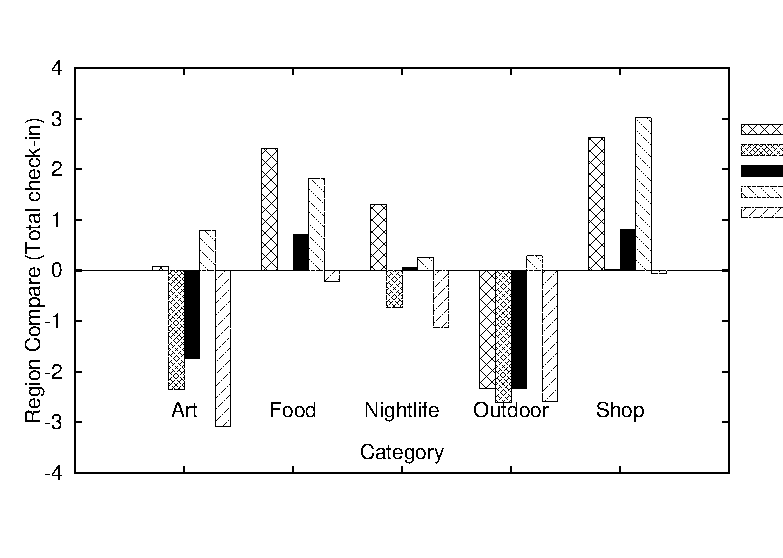
\epsfig{file=plot/RegionCompare.eps,width=0.7\columnwidth}
% figure caption is below the figure
\caption{Region Compare (Total Check in)}
\label{fig:RC}       % Give a unique label
\end{figure}

\begin{figure}[ht]
\centering
% Use the relevant command to insert your figure file.
% For example, with the graphicx package use
  \epsfig{file=plot/F1_measure_using_RegCom_T_feature.eps,width=0.7\columnwidth}
% figure caption is below the figure
\caption{F1 measure using RegCom feature}
\label{fig:F1RC}       % Give a unique label
\end{figure}

\section{Name Feature}
Similarly with human guessing the category of POI, the first intuition we got from a POI is its name. We build NAME feature in a straight forward way. We break POI��s name into words, we collect all the words, and filter out those showed up in only one POI. Then the words build up a dictionary, and NAME feature is binary representation of POI��s name in the dictionary.

\section{Experiment}
In order to prove the effectiveness of spatial features, we test the features on NAME, NAME+BASE, NAME+BASE+BEST. We use LIBLINEAR, one of the most popular classification toolkits, to build a binary classifier for each category, and then combine the result of the classifiers to produce the final classification result.

In the following, we introduce our data set first, and start by testing features individually on different categories to show different strength of features on different categories, then we show the result after choosing the best combination of features for each category. In the last two parts, we combine the results of categories' binary classifiers to produce multi-label result for Level 1 category and Level 2 categories.

\subsection{Data set description}
In order to test spatial features, we select check-ins from Foursquare in cities of two different size: NewYork(7817 POIs, 20885 check-ins), Singapore(38394 POIs,367570 check-ins). We use category hierarchy from Foursquare, too, we show the first level categories and their percentage in the two data set in Table \ref{tab:CategoryInfo}, and later we also do experiments on second level category, which is more specified including 278 categories. Among the POIs, there are 15.9\% of NewYork and 11.5\% of Singapore that are with multiple labels. We show that spatial features influenced less by user check-ins and consistently show improvements over BASE features.

\begin{table}
% Table generated by Excel2LaTeX from sheet 'Sheet1'
\caption{Please write your table caption here}
\label{tab:CategoryInfo}
\begin{tabular}{|c|r|r|}
\hline
 & NewYork(7817) & Singapore(38394) \\
\hline
Arts \& Entertainment &       10\% &        5\% \\
\hline
College \& University &        3\% &        8\% \\
\hline
      Food &       40\% &       28\% \\
\hline
Nightlife Spot &       19\% &        4\% \\
\hline
Outdoors \& Recreation &        4\% &        6\% \\
\hline
Professional \& Other Places &       16\% &       18\% \\
\hline
 Residence &        4\% &       16\% \\
\hline
Shop \& Service &       18\% &       19\% \\
\hline
Travel \& Transport &        5\% &        9\% \\
\hline
\end{tabular}


\end{table}

\subsection{Features on different Categories}
We show different features' strength on different categories in Fig. \ref{fig:F1FeatureCate}. One thing to be noted here is that even some features do not work well on their own, they show some different aspects of the POI, thus still can improve result.

We start by seeing BASE feature's performance over others in different categories. BASE feature consists of user behavior analysis, it works very well on Nightlife Spot and Professional \& Other Places, which has typical time characteristic, at night and on weekday individually. However, it works not so well on places with less characteristic on time specifically, for example Arts \& Entertainment, Shop \& Service.

NB\_m feature showed relatively good result among all the categories, showing that most of the POIs appear at appropriate and typical neighborhood for them. Interesting fact about N\_k feature is that it will get significant better result than NB\_m when POIs of same category gathering ''purely"" together, such as College \& University and Residence, however not so good result when the category normally mixed with other categories, such as Nightlife Spot. When using N\_K feature alone, the performance rely largely on whether the POIs near are within the same category. LCD feature, which measures distance to different categories, on its own is a very weak feature. When using it alone, it will show accordance with N\_k feature. The reason is that LCD get small distance to the POIs with same category, thus has similar effect as N\_K feature. Region compare on total check-in and unique user have similar effect.


\begin{figure}[h]
\centering
\subfigure[Arts \& Entertainment]{
\label{fig:F1FeatureArt}
\epsfig{file=plot/Graph_Youer/FeatureF1ForCate_data/Arts_&_Entertainment_data.eps,width=0.3\columnwidth}
}
\subfigure[Shop \& Service]{
\epsfig{file=plot/Graph_Youer/FeatureF1ForCate_data/Shop_&_Service_data.eps,width=0.3\columnwidth}
}
\subfigure[Food]{
\epsfig{file=plot/Graph_Youer/FeatureF1ForCate_data/Food_data.eps,width=0.3\columnwidth}
}
\subfigure[Nightlife Spot]{
\epsfig{file=plot/Graph_Youer/FeatureF1ForCate_data/Nightlife_Spot_data.eps,width=0.3\columnwidth}
}
\subfigure[Outdoors \& Recreation]{
\epsfig{file=plot/Graph_Youer/FeatureF1ForCate_data/Outdoors_&_Recreation_data.eps,width=0.3\columnwidth}
}
\subfigure[Professional \& Other Places]{
\epsfig{file=plot/Graph_Youer/FeatureF1ForCate_data/Professional_&_Other_Places_data.eps,width=0.3\columnwidth}
}
\subfigure[College \& University]{
\epsfig{file=plot/Graph_Youer/FeatureF1ForCate_data/College_&_University_data.eps,width=0.3\columnwidth}
}
\subfigure[Residence]{
\epsfig{file=plot/Graph_Youer/FeatureF1ForCate_data/Residence_data.eps,width=0.3\columnwidth}
}
\subfigure[Travel \& Transport]{
\epsfig{file=plot/Graph_Youer/FeatureF1ForCate_data/Travel_&_Transport_data.eps,width=0.3\columnwidth}
}
\caption{F1 score for individual features on categories}
\label{fig:F1FeatureCate}
\end{figure}







\subsection{Choosing feature parameter and combination}
As mentioned above, different parameter would have different effect on classification of different categories.Moreover, different combinations of parameters will also result in different accuracy. Thus, we tried all possible combinations for different categories and choose the best one based on tune set, and get the experiment result on the test set.

In the experiment on NewYork's data, every category gets better result over NAME+BASE except Art \& Entertainment, which results from the imbalance from test set and tune set, the best combination we choose for Art for NewYork works very well on tune set while not so well on test set.

In the experiment on Singapore's data, all the categories get better result over NAME+BASE, which benefit from the abundant train data.

Concluding from the two results on each category, we find that adding up spatial features will help in identifying a POI's category, but which features to add depend on the characteristic of the particular category.

%\begin{figure}[h]
%\centering
%\subfigure[NewYork]{
%\epsfig{file=plot/Graph_Youer/NewYorkF1.eps,width=0.47\columnwidth}
%}
%\subfigure[Singapore]{
%\epsfig{file=plot/Graph_Youer/SingaporeF1.eps,width=0.47\columnwidth}
%}
%\end{figure}

\begin{figure}[h]
\centering
% Use the relevant command to insert your figure file.
% For example, with the graphicx package use
  \epsfig{file=plot/Graph_Youer/NewYorkF1.eps,width=0.7\columnwidth}
% figure caption is below the figure
\caption{F1 score of different categories(NewYork)}
\label{fig:NewYorkF1}       % Give a unique label
\end{figure}
\begin{figure}[h]
\centering
% Use the relevant command to insert your figure file.
% For example, with the graphicx package use
  \epsfig{file=plot/Graph_Youer/SingaporeF1.eps,width=0.7\columnwidth}
% figure caption is below the figure
\caption{F1 score of different categories(Singapore)}
\label{fig:SingaporeF1}       % Give a unique label
\end{figure}

\subsection{Multi-label Classification Result}
We will get a prediction,indicating a 0-1 label for given category, and the probability output, indicating the probability of belonging to given category, from each category's classifier. We evaluate the prediction result by performing strict accuracy, precision and recall measure on multi-label classification. And we also produce a ranking list of the category label by probability output for each POI, we show ground-truth labels are ranked high in the ranking list to illustrate the reliability of candidate category labels we provide. We apply One-error, Coverage and average precision to measure the ranking list.
\subsubsection{Multi-label Performance Metrics}
\paragraph{Strict prediction measure} We define POI test set $T$ as a set of $|T|$ POI multi-label instances $(t_i, L_i)$, where $t_i$ is a POI, and $L_i$ is the ground-truth label set for $t_i$. The label(category) space $C$ consist of $|C|$ categories, for each category we have a binary classifier $BC_c, c \in C$. Each classifier have a 0-1 label for each instance $BC_j(t_i) = x, x \in {0,1}$, the final category prediction for $t_i$ is $P_i = \bigcup_{BC_c(t_i)=1} c \in C $,  Thus, we measure accuracy, precision and recall as follows.
\begin{description}
\centering
\item $Accuracy(T)=\frac{1}{|T|} \sum^{|T|}_{i=1} \frac{|L_i \cap P_i|}{|L_i \cup P_i|}$

\item $Precision(T)=\frac{1}{|T|} \sum^{|T|}_{i=1} \frac{|L_i \cap P_i|}{|P_i|}$

\item $Recall(T)=\frac{1}{|T|} \sum^{|T|}_{i=1} \frac{|L_i \cap P_i|}{|L_i|}$
\end{description}
\paragraph{Ranking list measure}
We further define probability of $t_i$ given category $c$ as $Pr_i(c)$. We have a permutation of C's items descending ordered by $Pr_i(c)$.
\begin{description}

\item[One-error:] Evaluation of whether ranked top category belongs to the ground-truth category set. $OneError = \frac{1}{|T|} \sum^{|T|}_{i=1}f([\arg\max_{c \in C} Pr_i(c)] \notin L_i$, for and predicate $\pi$, $f(\pi)$ equals 1 if $\pi$ holds and 0 otherwise.

\item[Coverage:] Evaluation of how many items should be seen on the list in order to cover all the ground-truth categories. We define $R_i(c)$ as the category c's rank in category ranking list of $t_i$. Thus  $Coverage = \frac{1}{|T|} \sum^{|T|}_{i=1} \max_{l \in L_i} R_i(l) -1$.

\item[Average Precision:] Evaluation of the ranking list considering all the positions that should belongs to ground-truth categories in the list. For each test instance $t_i$, $AveragePrecison_i = \sum_{j=1}^{j=|L_i|} \frac{I(j)*(n_j/j)}{|L_i|}$, where $n_j$ is the number of ground-truth category before the position $(j+1)$ in the ranking list, and $I(j)$ equals 1 if the category at position j belongs to $L_i$ and 0 otherwise. Then the $AveragePrecision = \frac{1}{|T|} \sum^{|T|}_{i=1} AveragePrecision_i$
\end{description}

\subsubsection{First Level Classification}
We first perform classification on First Level categories, including 9 categories as shown in Table \ref{tab:CategoryInfo}. Overall, adding spatial features would have better result on different measures except recall, which we believe reasonable to be prudent in labeling the POI a category. Comparing to NewYork, Singapore gains better result on all the three feature usage and show greater improvement with the spatial features, which largely benefits from larger dataset thus more feature instances and tenser POI distribution for spatial features.

 Good Average Precision indicating that category candidates for POI having multi-labels are reliable.

%\begin{figure}[h]
%\centering
%\subfigure[One Error]{
%\epsfig{file=plot/Graph_Youer/FirstClassOneError.eps,width=0.47\columnwidth}
%}
%\subfigure[Coverage]{
%\epsfig{file=plot/Graph_Youer/FirstClassCoverage.eps,width=0.47\columnwidth}
%}
%\caption{L1 Category Classification
%\end{figure}

\begin{figure}
\begin{minipage}[ht]{0.5\linewidth}
\centering
\includegraphics[width=\columnwidth]{plot/Graph_Youer/FirstClassOneError.eps}
\caption{L1 Classification One Error}
\label{fig:L1OneError}
\end{minipage}
\begin{minipage}[ht]{0.5\linewidth}
\centering
\includegraphics[width=\columnwidth]{plot/Graph_Youer/FirstClassCoverage.eps}
\caption{L1 Classification Coverage}
\label{fig:L1Coverage}
\end{minipage}
\end{figure}

\begin{figure}[h]
\centering
\hspace{-3cm}
\subfigure[NewYork]{
\epsfig{file=plot/Graph_Youer/FirstClassNewYork.eps,width=0.7\columnwidth}
}
\hspace{-3cm}
\subfigure[Singapore]{
\epsfig{file=plot/Graph_Youer/FirstClassSingapore.eps,width=0.7\columnwidth}
}
\hspace{-3cm}
\caption{L1 Category Classification overall Performance}
\label{fig:L1Overall}
\end{figure}


\subsubsection{Second Level Classification}
We further goes on with Second Level Classification, which includes more than 200 categories. Second level categories are more specific, for example, Shop \& Service are further split to Clothing Store, Bank and Gym / Fitness Center, etc.

One way to choose spatial features for second level categories is to inherit the feature combinations from their parent categories, which we applied. Choose the best from the top combinations of the parent category may also be a choice, but according to our experiment, the two way do not have much difference, but the first is significantly superior in time expense.

On this level, adding up BASE feature alone can not yield better result on NewYork anymore and no significant improvement on Singapore either, since the visiting time distribution are not so obvious with confidence any more on a specific category when the training data is not enough. But spatial features still works well, indicating that second level categories still have the spatial characteristics described by the spatial features we propose, and such characteristics are less likely to be diluted since POI's location suffer less by the randomness, and they are not so depend on user check-in data. As a result, performance improves on both NewYork and Singapore and not affected by the scale of data.


\begin{figure}[h]
\centering
\hspace{-3cm}
\subfigure[NewYork]{
\epsfig{file=plot/Graph_Youer/SecondClassNewYork.eps,width=0.7\columnwidth}
}
\hspace{-3cm}
\subfigure[Singapore]{
\epsfig{file=plot/Graph_Youer/SecondClassSingapore.eps,width=0.7\columnwidth}
}
\hspace{-3cm}
\caption{L2 Category Classification}
\end{figure}

\section{Conclusion}
In this paper, we propose a few-shot learning framework for relation classification that aims to extract information within support instances and using data augmentation. Our methods are extremely powerful under circumstances where limited training data is available.
%MME aims to extract underlying information brought within support sentences. In MME, a supplementary classifier is adopted to classify the relation of each support sentence, and participates in the back propagation progress by a fast-slow learner strategy. We also propose a way of aggregating cross-domain data into the training process. This helps the model to learn underlying cross-domain knowledge. These two innovations are especially useful under circumstances where extremely few data is available.
Additionally, we construct our own dataset, the TinyRel-CM dataset, a Chinese few-shot relation classification dataset in medical domain. The small training data size makes the TinyRel-CM dataset a challenging task.
%Different from previous released few-shot relation classification datasets, the TinyRel-CM dataset contains extremely limited labeled data and provides a much harder few-shot learning task. Our proposed MME framework and data augmentation method achieves state-of-the-art accuracy on the TinyRel-CM dataset and competitive results on the FewRel dataset.
%As for future work, we aim to extract abundant relation classes and instances from massive open-source data with our proposed MME framework to construct a knowledge base in medical domain .


%
%\section{Section title}
%\label{sec:1}
%Text with citations \cite{RefB} and \cite{RefJ}.
%\subsection{Subsection title}
%\label{sec:2}
%as required. Don't forget to give each section
%and subsection a unique label (see Sect.~\ref{sec:1}).
%\paragraph{Paragraph headings} Use paragraph headings as needed.
%\begin{equation}
%a^2+b^2=c^2
%\end{equation}
%
%% For one-column wide figures use
%\begin{figure}
%% Use the relevant command to insert your figure file.
%% For example, with the graphicx package use
%  \includegraphics{example.eps}
%% figure caption is below the figure
%\caption{Please write your figure caption here}
%\label{fig:1}       % Give a unique label
%\end{figure}
%%
%% For two-column wide figures use
%\begin{figure*}
%% Use the relevant command to insert your figure file.
%% For example, with the graphicx package use
%  \includegraphics[width=0.75\textwidth]{example.eps}
%% figure caption is below the figure
%\caption{Please write your figure caption here}
%\label{fig:2}       % Give a unique label
%\end{figure*}
%%
%% For tables use
%\begin{table}
%% table caption is above the table
%\caption{Please write your table caption here}
%\label{tab:1}       % Give a unique label
%% For LaTeX tables use
%\begin{tabular}{lll}
%\hline\noalign{\smallskip}
%first & second & third  \\
%\noalign{\smallskip}\hline\noalign{\smallskip}
%number & number & number \\
%number & number & number \\
%\noalign{\smallskip}\hline
%\end{tabular}
%\end{table}
%
%
%%\begin{acknowledgements}
%%If you'd like to thank anyone, place your comments here
%%and remove the percent signs.
%%\end{acknowledgements}
%
%% BibTeX users please use one of
%%\bibliographystyle{spbasic}      % basic style, author-year citations
%%\bibliographystyle{spmpsci}      % mathematics and physical sciences
%%\bibliographystyle{spphys}       % APS-like style for physics
%%\bibliography{}   % name your BibTeX data base
%
\bibliographystyle{spbasic}
\bibliography{reference}

%% Non-BibTeX users please use
%\begin{thebibliography}{}
%%
%% and use \bibitem to create references. Consult the Instructions
%% for authors for reference list style.
%%
%\bibitem{RefJ}
%% Format for Journal Reference
%Author, Article title, Journal, Volume, page numbers (year)
%% Format for books
%\bibitem{RefB}
%Author, Book title, page numbers. Publisher, place (year)
%% etc
%\end{thebibliography}

\end{document}
% end of file template.tex

